\chapter{Electron Cloud Build-up
Simulations}
\label{ch:1}

The first attempts to simulate the buildup of electron clouds in particle accelerators date back more than 20 years and many advancements have been done both in the physical modelling and the numerical algorithms needed for the simulations.
The majority of the past studies aimed at studying the electron cloud buildup mechanisms in longitudinally symmetric structures possibly with externally applied magnetic fields. Typical study cases are the long magnets of big particle accelerators, such as the CERN LHC or the SPS. In these cases several simplifications can be done to the physical models, thanks to which the complexity and the computational burden of the simulations can be reduced greatly. 
In this first chapter we would like to give an overview of these physical models and the numerical strategies in use in the main electron cloud buildup codes together with explanations of the assumptions and approximations that are made in the simulations. Moreover, we will show how these numerical methods can be extended and we will confirm the validity of the approximations which are traditionally made.

\section{The Electron Cloud Build-up Mechanism}
\label{sec:SEY}
The buildup of an electron cloud in a section of a particle accelerator is a well-studied mechanism and takes the name of multipacting effect. We give a schematic summary of how multipacting works:
\begin{BoxedText*}
\begin{itemize}
    \item Primary electrons are produced inside the beam pipe by residual gas ionization or photoemission due to synchrotron radiation;
    \item The electrons are accelerated by the passage of a proton bunch and hit the wall of the beam pipe;
    \item The impact of the electrons on the conducting beam pipe can result in the emission of new electrons;
    \item The newly emitted electrons can, in turn, be accelerated by the passage of the next proton bunch and the process can repeat resulting in an avalanche production of electrons;
\end{itemize}
\end{BoxedText*}
To understand the conditions under which the multipacting effect can happen it is important to model accurately the secondary emission mechanism, meaning that one has to specify a criteria to decide how many secondary electrons are emitted for every electron that impinges on the beam pipe. Several theoretical and experimental studies resulted in complex models which can take into account different material properties.\\
We summarize the secondary emission model in use at CERN, as it is the one we will use in all the studies carried out in this thesis.\\
A secondary emission models specifies a rule to compute the Secondary Emission Yield (SEY), which is defined as the ratio between the emitted and impinging current of electrons. In its simplest instance the SEY is a function of the energy of the impinging electrons $E$ and the angle of impact $\theta$
$$\delta(E, \theta) = \frac{I_{emit}}{I_{imp}(E, \theta)}.$$
The emitted current is composed of electrons which are elastically reflected and the true secondaries, which are the electrons that are actually ripped from the pipe, consequently the SEY is split into two contributions which have to be modelled separately
$$\delta(E, \theta) = \delta_{true}(E, \theta) + \delta_{elas}(E).$$
The component relative to the elastically reflected electrons depends solely on the impact energy and can be parameterized as
$$\delta_{elas}(E) = R_0 \left( \frac{ \sqrt{E} - \sqrt{E - E_0} }{ \sqrt{E} + \sqrt{E - E_0} } \right)^2 ,$$
where $R_0$ and $E_0$ encode the material properties.\\
For the component relative to the true secondaries we have the model,
\begin{equation*}
    \begin{split}
        \delta_{true}(E, \theta) &= \delta_{max}(\theta) \frac{ s_{true}\frac{E}{E_{max}(\theta)} }{s_{true} - 1 + \left( \frac{E}{E_{max}(\theta)}\right)^{s_{true}}}\\
        \delta_{max}(\theta) &= \delta_{max} e^{\frac{1-\cos(\theta)}{2}}\\
        E_{max}(\theta) &= E_{max} \left( 1 - 0.7(1 - cos(\theta)) \right)\\
    \end{split}
\end{equation*}
where $s_{true}$, $\delta_{max}$, $E_{max}$ are material-specific parameters.\\
The energies of the true secondary electrons are assumed to follow a log-normal distribution, i.e.
$$\frac{d n_{true}}{d E} = \frac{1}{E\sigma_{true} \sqrt{2 \pi}} e^{- \frac{(\ln(E)-\mu_{true})^2}{2 \sigma_{true}^2}},$$
while the angle of emission follows a cosine distribution.
In table \ref{tab:LHCVals} we report the values for the material parameters which are typically assumed for the LHC beam pipe and in Fig. \ref{fig:SEYcurves} we show the corresponding SEY curves. We don't specify a value for $\delta_{max}$ because this parameter depends on the past history of the material and it is influenced by several external factors. As a matter of fact, measurements have shown that this parameters varies significantly along the different sectors of the LHC for reasons that are not entirely clear. In Fig. \ref{fig:SEYcurvesdelta} we show the SEY curves for different values of $\delta_{max}$
\begin{table}
\begin{tabular}{c c}
    \hhline{==}
    Parameter & Value\\
    \hline
    $R_0$ &  0.7\\
    $E_0$ &  150eV\\
    $s_{true}$ & 1.35\\
    $E_{max}$ & 332eV \\
    $\mu_{true}$ & 1.6636\\
    $\sigma_{true}$ & 1.0828\\
    \hhline{==}
\end{tabular}
\caption{The values of the material parameters for the LHC beam pipe.}
\label{tab:LHCVals}
\end{table}

\begin{figure}
     \centering
    \begin{subfigure}[b]{0.4\textwidth}
        \hspace*{-1cm}
        \centering
        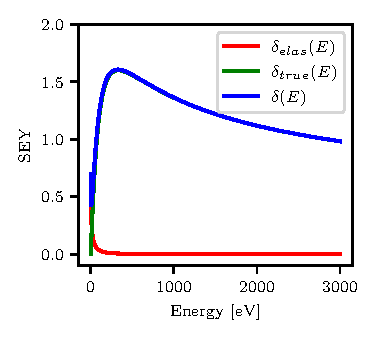
\includegraphics{chapters/Chapter1/Figures/SEY_components.pdf}
        %\caption{Caption}
    \end{subfigure}
    \hfill
    \begin{subfigure}[b]{0.4\textwidth}
        \hspace*{-1cm}
        \centering
        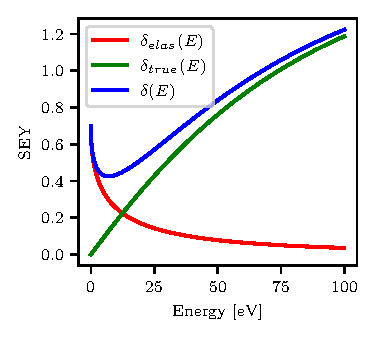
\includegraphics{chapters/Chapter1/Figures/SEY_components_zoom.pdf}
    \end{subfigure}
    \caption{The SEY curves corresponding to the material parameters of the LHC shown in table \ref{tab:LHCVals}. The right figure shows a zoom of the left one for low energies.}
    \label{fig:SEYcurves}
\end{figure}
\begin{figure}
    \centering
    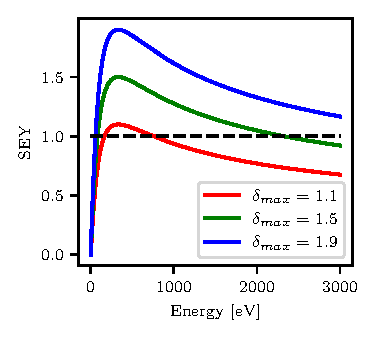
\includegraphics{chapters/Chapter1/Figures/SEY_delta_max.pdf}
    \caption{SEY curves for different values of $\delta_{max}$}
    \label{fig:SEYcurvesdelta}
\end{figure}


\begin{Remark}
Another secondary emission model, known as the Furman-Pivi model, has been developed in contemporary to the one used at CERN. This model is somewhat more complex than the one we reported as it also takes into account the rediffused electrons, which are back-scattered into the beam pipe after after losing some of their energy in the impact.
Historically, the Furman-Pivi model has been more popular in the American community and it has been implemented in POSINST, which is a 2D electrostatic buildup code.
In \cite{Wulff:2683285} it has been shown that the presence of rediffused electrons doesn't change substantially the simulation results so we decided to stick to the simpler model.
\end{Remark}

\begin{Remark}
As it has been described in \cite{Iadarola:thesis} there are a number of mechanisms that can lead to the production of primary electrons in the beam pipe of an accelerator. The focus of our simulations and studies is on the buildup of the electron cloud rather than on the production of primary electrons so in our simulations we will always start by introducing an uniform distribution of electrons in the chamber. This simplified strategy is justified by the fact that in the long run the electron cloud distribution is not affected by the how the primary electrons were produced.
\end{Remark}


\section{2D Electrostatic Simulations}
When the goal is to simulate the buildup of an electron cloud in a a long (almost) straight sector of a particle accelerator with static external fields it is possible to make some assumptions which simplify greatly the simulations.\\
The dimensionality of the domain can be reduced by assuming invariance along the longitudinal coordinate (we usually call it $s$) of the accelerator and the simulations are carried out in a transverse section of the domain of interest (the $x$-$y$ plane). In this type of simulations the electrons are still assumed to have a velocity along the s-axis, therefore they are some times referred to as 2D3V simulations. This approximation helps greatly to speed-up the simulations and it allows very refined studies even without the use of parallel computing, but indeed it cannot be made when simulating more complex structures. \\
In addition, usually the electrons are assumed to be slow enough for their field to be computed in the electrostatic approximation, even when they are accelerated by the field of the proton bunches. To the best of our knowledge a proper validation of the electrostatic approximation has never been done in the past, therefore we will verify its opportunity with simulation studies later in this chapter and in the next one. In particular, in Section \ref{sec:boostedFrame} we will show the validity of this assumption when studying electron clouds produced by ultra-relativistic beams in s-symmetric structures.\\
In the next section we will describe the procedure for the 2D electrostatic simulations implemented in PyECLOUD (a very similar one is implemented in POSINST).
The main algorithm in use is the particle-in-cell (PIC), which is often used to describe the evolution of systems of charged particles. The electrons are bundled in macro-particles to reduce the computational complexity, while the domain of the simulation is discretized using a square cartesian regular mesh. At every time step the charge of the macro-particles is interpolated (or scattered) to the mesh nodes. The nodal charge density is then used as a source of a Poisson problem solving which we obtain the electrostatic potential. The electric field on the mesh is then computed as the gradient of the electrostatic potential and it is then interpolated (gathered) at the positions of the MPs which are then pushed by integrating their equations of motions. We now give detailed explanations of each of the steps of the algorithm.
\subsection{Charge Scatter}
\label{subsec:chargescatter}
Let us refer to the situation where we have $N_{MP}$ MPs each of which lies at the position $(x_{p}, y_{p})$ for $p = 1, \dots, N_{MP}$. We are going to interpolate their charges $\rho_p$ to the mesh nodes using the so-called area weighting algorithm. If a MP lies in the cell $(i, j)$ its position in the cell is defined by 
\begin{equation}\label{eq:dxdy}
    \begin{split}
        d^p_x &= x_p - (x_0 + i \Delta h)\\
        d^p_y &= y_p - (y_0 + j \Delta h)
    \end{split}
\end{equation}
where $\Delta h$ is the mesh width and $(x_0, y_0)$ is the bottom left corner of the mesh. To find indices $i$ and $j$ of the cell containing the point $(x_{p}, y_{p})$ we have the simple formulae
\begin{equation*}
    \begin{split}
        i &= \left\lfloor \frac{x_p - x_0}{dh} \right\rfloor,\\
        j &= \left\lfloor  \frac{y_p - y_0}{dh} \right\rfloor.
    \end{split}
\end{equation*}
Then every particle contributes to the nodal charge density as follows:
\begin{align*}
    \rho_{i, j} &= \rho_{i, j} + \rho_p \left(1 - \frac{d_x^p}{\Delta h}\right)\left(1 - \frac{d_y^p}{\Delta h}\right),\\
    \rho_{i + 1, j} &= \rho_{i + 1, j} + \rho_p \frac{d_x^p}{\Delta h}\left(1 - \frac{d_y^p}{\Delta h}\right),\\
    \rho_{i, j + 1} &= \rho_{i, j + 1} + \rho_p \left(1 - \frac{d_x^p}{\Delta h}\right)\frac{d_y^p}{\Delta h},\\
    \rho_{i + 1, j + 1} &= \rho_{i + 1, j + 1} + \rho_p \frac{d_x^p}{\Delta h} \frac{d_y^p}{\Delta h}.\\
\end{align*}
It is easy to show that this procedure is charge conserving, meaning that $$\sum_{i=1}^{N_x}\sum_{i=1}^{N_y} \rho_{i, j} = \sum_{p = 0}^{N_{MP}} \rho_p.$$

\subsection{Electron Cloud Self-Fields Computation}
\label{subsec:ecloudfield}
As already mentioned, the self-fields of the electron cloud (also called the electron cloud space-charge fields), are assumed to be slow-varying. In addition we also assume s-symmetry, therefore by dropping all the temporal and longitudinal derivatives from the Maxwell's equations we obtain 
\begin{align*}
    \nablaxy \cdot \mathbf{E} &= \frac{\rho}{\varepsilon_0},\\
    \nablaxy \times \mathbf{E} &= \mathbf{0}.
\end{align*}
with the transverse nabla operator $\nablaxy = (\frac{\partial}{\partial x}, \frac{\partial}{\partial y})^T$.
The second equation implies that the electric field can be expressed as $$\mathbf{E} = \nablaxy \phi,$$ where $\phi$ is the electrostatic potential. Plugging this expression into the first equation (the Gauss law) we obtain the Poisson problem 
\begin{align*}
    \begin{cases}
        \lapxy \phi&= \frac{\rho}{\varepsilon_0} \quad \mathrm{in} \ \Omega,\\
        \phi&= 0 \quad \mathrm{outside} \ \mathrm{of} \ \Omega,
    \end{cases}
\end{align*}
where $\Omega$ is a section of the beam pipe. We constraine $\phi$ to zero outside on the surface of chamber because we model the pipe as a perfect electric conductor (PEC). Moreover, since we assume that the pipe shields perfectly the exterior area, we set the potential to zero also everywhere outside the chamber.
In order to find the potential $\phi$ numerically we discretize it at the mesh nodes, i.e.
$$\phi_{i, j} = \phi(i \Delta h + x_0, j \Delta h + y_0),$$ and, use a centered discretization for the Laplace operator, the Poisson equation becomes $${\lapxy}_{,h} \phi_{i,j} = \frac{\phi_{i-1, j} + \phi_{i, j - 1} - 4\phi_{i,j} + \phi_{i + 1, j} + \phi_{i, j + 1}}{\Delta h^2} = -\frac{\rho_{i, j}}{\varepsilon_0}.$$
for every $i = 1, \dots ,N_x$ and $j = 1, \dots, Ny$ such that $(i\Delta h + x0, j\Delta h + y0) \in \Omega$.
On the other hand to take into account the boundary condition we have to impose $$\phi_{i,j} = 0$$
for every $i = 1, \dots ,N_x$ and $j = 1, \dots, Ny$ such that $(i\Delta h + x0, j\Delta h + y0) \notin \Omega$.\\
The $\phi_{i, j}$'s and the $\rho_{i,j}$'s can be arranged in a lexicographic order to form the vectors $\boldsymbol{\phi}, \boldsymbol{\rho} \in \mathbb{R}^{N_xN_y}$ and the discrete problem can be cast as a system of linear equation $$\mathbf{A}\boldsymbol{\phi} = \boldsymbol{\rho}.$$
The matrix $\mathbf{A}$ is highly sparse, therefore it can be efficiently inverted directly using an LU decomposition.\\
Once $\phi$ is known it's possible to retrieve $\mathbf{E}$ using a centered discretization of $\nablaxy\boldsymbol{\phi}$:
\begin{equation*}
    \mathbf{E}_x|_{i,j} = \frac{\phi_{i+1,j} - \phi_{i-1,j}}{2\Delta h} \qquad 
    \mathbf{E}_y|_{i,j} = \frac{\phi_{i,j+1} - \phi_{i,j-1}}{2\Delta h}
\end{equation*}
When the boundaries of $\Omega$ do not conform to the mesh, for example if they are curved, the simple centered approximation is unable to resolve correctly the shape of the conductor resulting in a stair-cased approximation, as shown in figure \ref{fig:SCvsCutCell} for the case of a circle.
\begin{figure}
        \centering
        \includestandalone[width=0.5\textwidth]{chapters/Chapter1/Latex_Images/circle_staircase}
        \caption{Approximation of a circle (red) with a staircased (blue) and a cut-cell (green) approach.}
        \label{fig:SCvsCutCell}
\end{figure}
In such cases it is known that the accuracy of the method degrades to first order. The stencil can be modified to resolve properly the curved boundaries using the Shortley-Weller method \cite{ShortleyWeller}, in which the discrete derivatives are modified when their stencil would cross the PEC boundary. To begin with, each edge of the grid is associated with a length, which is $\Delta h$ if the edge is completely outside of the conductor, 0 if the edge is inside the conductor, or the length of the portion outside the conductor if the edge crosses the conductor boundary (i.e. the distance from the edge extreme point which lies outside the PEC and the PEC surface). Then, the new approximation of the Laplace operator reads:
\begin{align*}
    {\lapxy}_h^{SW} \phi_{i,j} = & \left(\frac{2}{l_x|_{i-1,j} l_x|_{i,j}} + \frac{2}{l_y|_{i,j-1} l_y|_{i,j}}\right)\phi_{i,j}\\
    &- \frac{2}{l_x|_{i, j}(l_x|_{i-1, j} + l_x|_{i, j})}\phi_{i+1,j}\\
    &- \frac{2}{l_x|_{i-1, j}(l_x|_{i-1, j} + l_x|_{i, j})}\phi_{i - 1,j}\\
    &- \frac{2}{l_y|_{i, j}(l_y|_{i, j-1} + l_y|_{i, j-1})}\phi_{i,j+1}\\
    &- \frac{2}{l_y|_{i, j-1}(l_y|_{i, j-1} + l_y|_{i, j})}\phi_{i,j-1}.
\end{align*}
The centered 5-points stencil and the Shortley-Weller cut-cell stencils are shown in Fig. \ref{fig:lapStencils}.
\begin{figure}
    \begin{subfigure}{0.45\linewidth}
        \centering
        \includestandalone{chapters/Chapter1/Latex_Images/laplacian_stencil}
    \end{subfigure}
    \hfill
    \begin{subfigure}{0.45\linewidth}
        \centering
        \includestandalone{chapters/Chapter1/Latex_Images/laplacian_stencil_cut}
    \end{subfigure}
    \caption{The numerical stencils for the laplacian computation. Left: the standard centered stencil. Right: an example of Shortley-Weller cut-cell stencil for a node adjacent to a conductor (the blue area).}
    \label{fig:lapStencils}
\end{figure}
When all the involved edges do not cross the PEC boundary then we find that ${\lapxy}_h^{SW} = {\lapxy}_h$.
The gradient computation is also modified and the electric field is found as
\begin{align*}
    \mathbf{E}_x|_{i,j} &= \frac{\phi_{i+1,j} -  \phi_{i,j}}{l_x|_{i,j}} + \frac{\phi_{i,j} -  \phi_{i-1,j}}{l_x|_{i-1,j}},\\
    \mathbf{E}_y|_{i,j} &= \frac{\phi_{i,j+1} -  \phi_{i,j}}{l_y|_{i,j}} + \frac{\phi_{i,j} -  \phi_{i,j-1}}{l_y|_{i,j-1}}.
\end{align*}
Also the gradient computation reduced to the classic centered one when when the stencil doesn't cross the PEC boundary.
For the nodes adjacent to the boundaries the Shortley-Weller approximation of the Laplacian operator is not centered, so locally the method has only first order of accuracy. On the other hand, it is possible to see that the Shortley-Weller is globally second order accurate \cite{weynans:ShortleyWellerOrder}.

\subsection{Field Gather}
Once the electric field is computed, it has to be interpolated at the particles position. In order for the energy of the system to be conserved the interpolation scheme has to be the same as for the scattering of electric charges. Therefore, for a MP at position $(x_p, y_p)$ which is located inside the cell $(i, j)$, the field is interpolated as
\begin{align*}
    \mathbf{E}_p = &\mathbf{E}_{i,j}\left(1-\frac{dx}{\Delta h}\right)\left(1-\frac{dy}{\Delta h}\right) +\\ &\mathbf{E}_{i+1,j}\frac{dx}{\Delta h}\left(1-\frac{dy}{\Delta h}\right) +\\
    &\mathbf{E}_{i,j+1}\left(1-\frac{dx}{\Delta h}\right)\frac{dy}{\Delta h} +\\
    &\mathbf{E}_{i+1,j+1}\frac{dx}{\Delta h}\frac{dy}{\Delta h}
\end{align*}
with $d_x^p$ and $d_y^p$ defined again as in \ref{eq:dxdy}.

\subsection{Macroparticle Push}
When only electromagnetic forces are considered the equations of motion of a particle describing its position position $\mathbf{r} = \begin{bmatrix} x(t)\\ y(t)\end{bmatrix}$ and velocity $\mathbf{v} = \begin{bmatrix} v_x(t)\\ v_y(t)\end{bmatrix}$ are
\begin{equation*}
    \begin{dcases}
        \frac{\partial \mathbf{r}}{\partial t} = \mathbf{v},\\
        \frac{\partial \mathbf{v}}{\partial t} = \mathbf{v} -\frac{q}{m}\left( \mathbf{E} + \mathbf{v}\times\mathbf{B} \right).
    \end{dcases}
\end{equation*}
The trajectory of each MP is influenced by the fields induced by the beam and by the other MPs and also by externally applied fields. In PyECLOUD it is possible to specify multipolar external fields which are defined according to the formula
\begin{equation*}
    B_y(x, y) + iB_x (x, y) = \sum_{k=0}^{N_B} \frac{1}{k!} (b_k + i b_k')(x+iy)^k.
\end{equation*}
For example, with this formalism a horizontally bending dipole magnet is defined taking $N_B = 0$ and having $b_0' = 0$. Then the magnetic field simplifies to
$$B_y(x, y) + iB_x(x, y) = b_1,$$
which yields $B_x = 0$ and $B_y = b_0$.\\
We compute the beam field separately from the electrons and we apply it as an external excitation. The details about the computation of the beam fields will be discussed in the next section.
Once the electromagnetic field at the position of each MP is known we can integrate numerically the equations of motion using as initial condition the positions and velocities at the current time step and find the positions and velocities at the next time step. PyECLOUD implements the Boris scheme without relativistic corrections as the electrons are assumed to travel well below the speed of light. We report the steps needed for the numerical integration of the equations of motion.\\
In the Boris algorithm the velocities and the speeds of the MPs are staggered by half a time step in time and, by using a leapfrog scheme, one obtains the discrete equations of motion
\begin{equation*}
    \begin{dcases}
        \frac{\mathbf{r}^{n+1}_p - \mathbf{r}^n_p}{\Delta t} = \mathbf{v}^{n+\half}_p,\\
        \frac{\mathbf{v}^{n+\half}_p - \mathbf{v}^{n-\half}_p}{\Delta t} = -\frac{q}{m}\left( \mathbf{E}_p + \bar{\mathbf{v}}\times\mathbf{B}_p \right),
    \end{dcases}
\end{equation*}
where $\bar{\mathbf{v}}$ is the averaged velocity $$\frac{\mathbf{v}^{n+\half}_p + \mathbf{v}^{n-\half}_p}{2}.$$
Since $\mathbf{v}^{n+\half}_p$ appears in both sides of the second equation the update equation for $\mathbf{v}^{n+\half}$ is still implicit. An explicit update equation is more computationally efficient, for this reason we need a rule to compute $\mathbf{v}^{n+\half}_p$. In the Boris algorithm, one splits the contributions coming from the electric and the magnetic fields by making the substitutions
\begin{equation}
    \label{eq:subsv}
    \begin{split}
        \mathbf{v}^{n-\half}_p &= \mathbf{v}^- - \frac{q}{m}\mathbf{E}_p \frac{\Delta t}{2},\\
        \mathbf{v}^{n+\half}_p &= \mathbf{v}^+ + \frac{q}{m}\mathbf{E}_p \frac{\Delta t}{2},
    \end{split}
\end{equation}
which lead to
\begin{equation*}
    \frac{\mathbf{v}^+_p - \mathbf{v}^-_p}{\Delta t} = \frac{q}{2m} \left(\mathbf{v}^+_p + \mathbf{v}^-_p \right) \times \mathbf{B}_p.
\end{equation*}
Multiplying both sides by $\left(\mathbf{v}^+_p + \mathbf{v}^+_p)\right)$ we find out $(\mathbf{v}^+_p)^2 = \mathbf{v}^-_p)^2$ showing that this equation defines $\mathbf{v}^+_p$ as a rotation around $\mathbf{B}_p$. Assuming that $\Delta t$ is small enough the rotation can be linearized and one finds that
\begin{equation}
\label{eq:v+}
\begin{split}
    \mathbf{v}'_p &= \mathbf{v}^-_p + \mathbf{v}^-_p\times\mathbf{t}_p,\\
    \mathbf{v}^+_p &= \mathbf{v}'_p + \mathbf{v}'_p-\times\mathbf{s}_p,
\end{split}    
\end{equation}
where
\begin{equation}
\label{eq:t&s}
\begin{split}
    \mathbf{t}_p &= \frac{q\mathbf{B}_p}{m} \frac{\Delta t}{2},\\
    \mathbf{s}_p &= \frac{2\mathbf{t}_p}{1+t^2}.
\end{split}    
\end{equation}
Now that have all the elements in place, we give the algorithmic steps to advance the position and velocity of a MP:
\begin{enumerate}
    \item compute the vectors $\mathbf{t}_p$ and $\mathbf{s}_p$ as prescribed by Eq. \ref{eq:t&s};
    \item compute $\mathbf{v}^+$ as in \ref{eq:v+};
    \item use the substitutions \ref{eq:subsv} to obtain $\mathbf{v}^{n+\half}$;
    \item advance the MP position with the leapfrog scheme $$\mathbf{r}_p^{n+1} = \mathbf{r}_p^n + \Delta t \mathbf{v}_p^{n+\half};$$
\end{enumerate}
the procedure is repeated for every MP obtaining the full electron cloud distribution at the time step $n+1$.
When dealing only with static multipolar magnetic fields, semi-analytic approaches like the one described in \cite{Iadarola:thesis} allow using larger time steps than the Boris algorithm thus reducing the number of time steps in a simulation. On the other hand, the Boris approach is very general and works well also when no external magnetic field is applied. In PyECLOUD both the semi-analytical algorithm and the Boris pusher are implemented but for our simulations we will always use the latter to be consistent with the approach we will use in Chapter 2 REF.
In PyECLOUD it is possible to do sub-stepping for the particle pusher so that the field computation is not performed every time that the particles are pushed. This is again justified by the fact that the electrons are assumed to move slowly and the potential doesn't change significantly at every time step.
\subsection{Problem-specifc matters}
In the previous sections we described algorithms which are generally common to any electrostatic PIC simulation. In this section we would like to discuss those that are specific to Electron Cloud buildup studies.
\subsubsection{The Beam Field}
The beam is assumed to be rigid, which means that the effect of the electron cloud on the beam is neglected. The beam distribution $\rho^{beam}$ can be separated between a transverse component $\rho^{beam}_{\perp}$ and a longitudinal component $\lambda$. The beam is also assumed to travel at the speed of light, with $\beta^{beam} = 1$, therefore we can write
$$\rho^{beam}(x, y, s) = \rho^{beam}_{\perp}(x, y)\lambda(s - c t).$$
The electromagnetic field of a beam travelling at the speed of light is known to be fully transverse to the direction of motion, i.e.
$$\mathbf{E}^{beam}\cdot\hat{\mathbf{i}}_s = \mathbf{B}^{beam}\cdot\hat{\mathbf{i}}_s = 0,$$ and $\mathbf{E}$ and $\mathbf{B}$ are related to each other through the formula $$\mathbf{B}^{beam} = \frac{\hat{\mathbf{i}}_s\times\mathbf{E}^{beam}}{c},$$ which yields 
\begin{equation}
    \label{eq:EBbeam}
    ||\mathbf{B}^{beam}|| = \frac{||\mathbf{E}^{beam}||}{c}.
\end{equation}
The force acting on an electron $\mathbf{F}^{beam}$ can be split into an electric and a magnetic contribution $$\mathbf{F}^{beam} = \mathbf{F}^{beam}_{\mathbf{E}} + \mathbf{F}^{beam}_{\mathbf{B}},$$
with $$\mathbf{F}^{beam}_{\mathbf{E}} = \frac{q}{m}\mathbf{E}^{beam},$$ and $$\mathbf{F}^{beam}_{\mathbf{B}} = \frac{q}{m}\left(\mathbf{v}_e\times\mathbf{B}^{beam}\right),$$
where $\mathbf{v}_e$ is the velocity of the electron. Hence, using Eq. \ref{eq:EBbeam} we obtain the following relation
\begin{equation*}
    \begin{split}
        ||\mathbf{F}^{beam}_{\mathbf{B}}|| &= \frac{q}{m} ||\mathbf{v}_e||||\mathbf{B}^{beam}|| \\
                                           &= \frac{q}{m} ||\mathbf{E}^{beam}|| \frac{||\mathbf{v}_e||}{c} = ||\mathbf{F}^{beam}_{\mathbf{E}}|| \frac{||\mathbf{v}_e||}{c}.
    \end{split}
\end{equation*}
In \cite{Iadarola:thesis} it is shown that the speed of the electrons is way smaller than the speed of light, therefore we can assume $$\mathbf{F}^{beam}_{\mathbf{B}} \approx 0,$$
and avoid the magnetic field computation.\\
The electric field computation can be simplified as shown in \cite{Iadarola:boostedframe} by showing that it holds
$$\mathbf{E}^{beam}(x, y, s, t) = \mathbf{E}_\perp^{beam}(x, y) \lambda(s - ct)$$
and
\begin{equation*}
    \begin{cases}
        \nablaxy \times \mathbf{E}^{beam}_\perp = 0,\\
        \nablaxy \cdot \mathbf{E}^{beam}_\perp = \frac{\rho_\perp^{beam}}{\varepsilon_0}.
    \end{cases}
\end{equation*}
Therefore, also the beam the electric field can be obtained as the gradient of a scalar potential $\phi^{beam}$ which is the solution of the Poisson problem
\begin{align*}
    \begin{cases}
        \lapxy \phi^{beam}&= \dfrac{\rho_\perp^{beam}}{\varepsilon_0} \quad \mathrm{in} \ \Omega,\\
        \phi&= 0 \quad \mathrm{outside} \ \mathrm{of} \ \Omega.
    \end{cases}
\end{align*}
This is very convenient because we can reuse the same Poisson solver as we did to compute the fields of the electrons and of the beam.\\
\begin{Remark}
Both for the beam and the electrons we need to solve a Poisson problem to compute the respective electric fields, but the reason for which the Maxwell's equations reduce to the Poisson problem are very different in the two cases. In the case of the electrons it is thanks to the electrostatic approximation, while for the beam it is thanks to the symmetry of the problem and to the fact that the beam is ultra-relativistic.
\end{Remark}

\subsubsection{Impacts and Secondary Emission}
Whenever a MP impinges on the surface of the beam pipe we need to compute the secondary emission information according to the model we reported in section \ref{sec:SEY} in order to determine know how many electrons should be reintroduced in the simulation.\\
The chamber is described as a polygon, therefore it is easy to check if a MP lies inside or outside the boundary. At every time step, the position of the MPs is checked and if a MP is found outside the chamber, its position of impact is computed by intersecting the boundary with the segment joining the current and the previous position of the particle. Besides the point of impact we also need to compute the normal to chamber surface in order to obtain the angle of impact.
Whenever a MP impacts on the beam-pipe, some electrons can be absorbed or emitted, therefore the weight of the MP is adjusted accordingly. In order to avoid having MPs with an excessively large MPs if the weight exceeds a threshold the MP is split into two.
\subsubsection{Management of the MPs}
As we've seen in the previous section, in an electron cloud buildup simulation the number of MPs and their weights can vary during time. Especially during phases of exponential blow-up of the number of electrons, the number of MPs will also tend to increase exponentially, increasing dramatically the amount of computations needed at every time step. In order to keep the number of MPs under control, every time that it exceeds a given threshold  we perform a re-sampling procedure called \textit{regeneration} (also referred to as culling) thanks to which the number of MPs is decreased to a pre-defined target.
The steps performed in a regeneration are the following:
\begin{BoxedText*}
\begin{enumerate}
    \item Determine the number of MPs to be culled $N_{cull}$ as the difference between the current number of MPs $N_{MP}$ and the target $N_{target}$;
    \item For every MP draw a random number from a $Poisson\left(\dfrac{N_{cull}}{N_{MP}}\right)$ distribution to decide whether it has to be suppressed;
    \item Redistribute uniformly the charge of the culled MPs among the other MPs;
\end{enumerate}
\end{BoxedText*}

At the end of this process the number of the MPs is reduced but the total charge is conserved.\\

\section{The Electron Cloud Saturation}
The numerical tools presented so far can be used for very advanced simulations of the electron cloud dynamics. In particular, in this section we will focus on studying the electron cloud saturation mechanism. It is well-known that during the passage of a train of bunches there is an exponential growth of the number of electrons which slows down and saturates in the long run. In Fig. \ref{fig:nel_timep} we show a typical example of the time evolution of the number of electrons in a circular pipe during the passage of a train of 100 bunches without external magnetic fields. 
\begin{figure}
\RawFloats
\begin{minipage}[c]{0.5\linewidth}
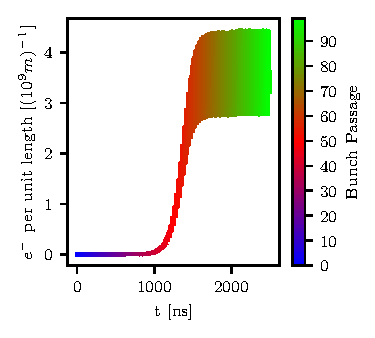
\includegraphics[scale=1.4]{chapters/Chapter1/Figures/nel_timep_sat.pdf}
\caption{The time evolution of the number of electrons in a circular beam pipe. \linebreak}
\label{fig:nel_timep}
\end{minipage}
\hfill
\begin{minipage}[c]{0.5\linewidth}
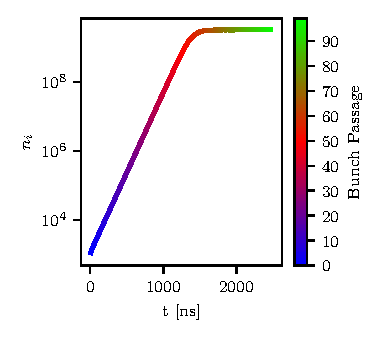
\includegraphics[scale=1.4]{chapters/Chapter1/Figures/nel_bunch_sat.pdf}
\caption{The number of electrons in the chamber after each time passage (in logarithmic scale).}
\label{fig:nel_bunch}
\end{minipage}%
\end{figure}

In this case we clearly see that after an initial exponential growth the number of electrons saturates around $3\cdot10^9$.
Before studying this phenomenon we show that the results of this type of study are stable under mesh refinement. In Fig. \ref{fig:scan_dh} it is possible to see that the multipacting curve converges as we decrease the mesh width $dh$.
\begin{figure}
    \centering
    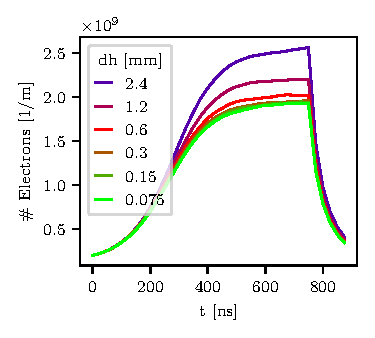
\includegraphics[scale=1.4]{chapters/Chapter1/Figures/scan_dh.pdf}
    \caption{Time evolution of the number of electrons in a circular pipe without external fields for increasing mesh resolutions.}
    \label{fig:scan_dh}
\end{figure}
To begin with we give a very brief mathematical description of the buildup process.\\
If $n_i$ is the number of electrons in the chamber after every bunch passage, we define a coefficient $\delta_{eff, i}$  such that $$n_{i+1} = \delta_{eff, i} n_i.$$
As shown in Fig. \ref{fig:nel_bunch}, typically $\delta_{eff, i}$ assumes a constant value larger than one during the exponential growth of the number of electrons and it suddenly transitions to one when the saturation stage begins.
\begin{figure}
    \centering
    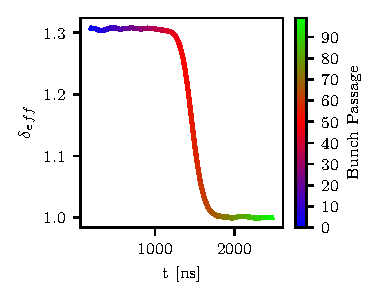
\includegraphics[scale=1.4]{chapters/Chapter1/Figures/delta_eff.pdf}
    \caption{The evolution of $\delta_{eff}$ during a electron cloud buildup simulation}
    \label{fig:delta_eff}
\end{figure}
Both in the exponential growth and in the saturation regime $\delta_{eff, i}$ takes constant values, which means $\delta_{eff, i} = \delta_{eff}$.
We treat separately the two regimes:
\begin{enumerate}
    \item $\delta_{eff}>1$: exponential growth. It is easily seen that $$n_{i+1} = \delta_{eff}^i n_1,$$
    showing the exponential dependence of $n_i$ on $i$.
    \item $\delta_{eff} = 1$: saturation. In this case we have $$n_{i+1} = n_{i},$$ hence the number of electrons stays constant.
\end{enumerate}
In the following we characterize the conditions that cause the transition from the exponential growth to the saturation.\\
In Fig. \ref{fig:exp_vs_sat_snap} we compare the distribution of the electrons during the two regimes.
\begin{figure}
    \centering
    \begin{subfigure}{0.47\textwidth}
        %\centering
        \hspace*{-2cm}
        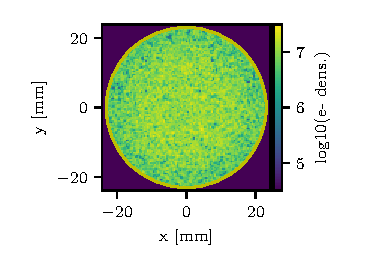
\includegraphics[scale=1.4]{chapters/Chapter1/Figures/edist_exp.pdf}
    \end{subfigure}
    %\hfill
    \begin{subfigure}{0.47\textwidth}
    
        %\centering
        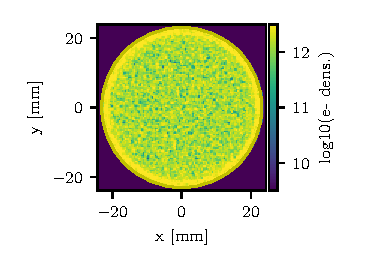
\includegraphics[scale=1.4]{chapters/Chapter1/Figures/edist_sat.pdf}
    \end{subfigure}
    \caption{Snapshots of the electron cloud distribution in an LHC dipole after a bunch passage during the exponential growth (left) and at saturation (right).}
    \label{fig:exp_vs_sat_snap}
\end{figure}
During the exponential growth the electrons populate rather uniformly the beam chamber, while at saturation they concentrate close to the beam pipe. The concentration of the electrons close to the boundary of the chamber is also seen very clearly in the radial position histograms in Fig. \ref{fig:hist_r_sat}.
\begin{figure}
    \centering
    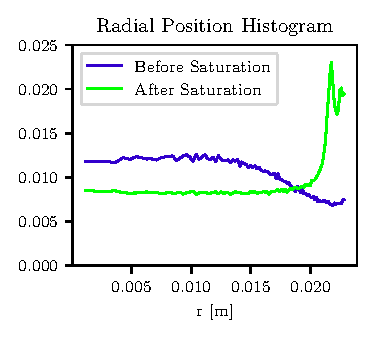
\includegraphics[scale=1.4]{chapters/Chapter1/Figures/hist_r.pdf}
    \caption{Radial position histograms of the electrons during the exponential growth (blue) and at saturation (green).}
    \label{fig:hist_r_sat}
\end{figure}
To explain this accumulation of electrons we first look at the profile of the electrostatic potential of the electrons in Fig. FIG. It is clear that at saturation electrons emitted with low energy don't manage to ``climb" the potential and remain concentrated close to the pipe. These electron that don't manage to reach the center of the cavity impinge against the pipe with low energies and are likely to be absorbed before a new bunch passage.
On the other hand, during the exponential growth even an electron with low energy can reach the center of the cavity and does not impinge on the wall until it is accelerated by the passage of the new bunch hitting the wall with high energy and producing the emission of new electrons. During the exponential growth the emitted electrons electrons outnumber the absorbed ones resulting in a net increase, while at saturation there is a balance between emitted and absorbed electrons. In Fig. \ref{fig:Nel_sat_overlap} we show the number of electrons in the pipe during different bunch passages divided by $n_i$. It is very clear that before saturation more electrons are emitted then absorbed, while at saturation ($N_{bunch}=95$) there is a perfect balance between emitted and absorbed electrons. 
\begin{figure}
    \centering
    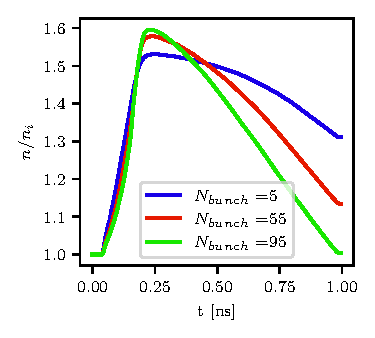
\includegraphics[scale=1.4]{chapters/Chapter1/Figures/nel_timep_sat_overlap.pdf}
    \caption{The number of electrons during a bunch passage $n$ relative to the number of electrons at the beginning of the passage $n_i$ for different bunch numbers.}
    \label{fig:Nel_sat_overlap}
\end{figure}
To further support our explanation, Fig. \ref{fig:lifetime_hist} we report the normalized distribution of the lifetimes of the electrons during the two phases. Here the lifetime is defined as the time elapsed between successive impacts of the electrons against the wall. In both cases a large fraction of the electrons survive for $25ns$, which exactly the bunch space. These are the electrons that produce most of the secondary emission. At saturation a much large fraction of electrons have a short lifetime and these electrons are likely absorbed.

\begin{figure}
    \centering
    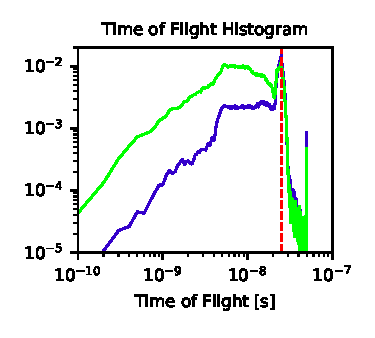
\includegraphics[scale=1.4]{chapters/Chapter1/Figures/lifetime_hist.pdf}
    \caption{Caption}
    \label{fig:lifetime_hist}
\end{figure}

\section{Electromagnetic Space-Charge Fields - Boosted Frame Solver}
\label{sec:boostedFrame}
Throughout this chapter we assumed that the electrons motion is slow enough for their field to be approximated as electrostatic. This approximation is found also in other electron cloud studies but a rigorous justification has never been given.
We will adopt a very simple approach to validate the electrostatic assumption: we will implement a special electromagnetic solver and we will benchmark the results of an electromagnetic simulation against those of an electrostatic simulation.\\
Let us consider the situation of Fig. \ref{fig:refFrames} in which an ultra-relativistic proton bunch crosses an electron cloud which doesn't move along the $s$ coordinate. 
\begin{figure}
    \centering
    \includestandalone[width=0.75\textwidth]{chapters/Chapter1/Latex_Images/boosted_frame}
    \caption{A bunch (red) crossing an electron cloud (green) with their reference frames.}
    \label{fig:refFrames}
\end{figure}
We consider two reference frames frame: the lab frame, in which the electron cloud is not moving longitudinally and the bunch moves with speed $v_s = \beta c$, and the co-moving frame, in which the bunch is stationary and the electron cloud moves in negative direction.\\
\subsection{Lorentz transformations to the Boosted Frame}
For the derivation of the boosted frame approach we will transform quantities from the lab frame to the co-moving frame and vice-versa. 
In special relativity, four-vectors are special vectors of four components which can be transformed between the lab frame and a boosted frame using the Lorentz transformation. This means that any four-vector $\left(a_x, a_y, a_s, a_t\right)$ can be transformed using the following relations
\begin{equation*}
    \begin{cases}
        a_x' &= a_x\\
        a_y' &= a_y\\
        a_s' &= \gamma(a_s-\beta a_t)\\
        a_t' &=\gamma\left(a_t-\beta a_s\right)
    \end{cases},
\end{equation*}
and
\begin{equation*}
    \begin{cases}
        a_x &= a_x'\\
        a_y &= a_y'\\
        a_s &= \gamma(a_s'+\beta a_t')\\
        a_t &=\gamma\left(a_t'+\beta a_s'\right)
    \end{cases}.
\end{equation*}
We remark that in the transformation the transverse components $a_x$ and $a_y$ remain unchanged.\\
We will make use of the following four-vectors:
\begin{BoxedText*}
\begin{enumerate}
    \item The four-position: $\left(x,y,s,ct\right) = \left(\mathbf{r}, ct\right)$;
    \item The four-current: $\left(J_x, J_y, J_s, c\rho\right)$;
    \item The four-potential: $\left(A_x, A_y, A_s, \frac{\phi}{c}\right)$;
\end{enumerate}
\end{BoxedText*}
\subsection{Derivation of the Boosted-Frame Solver}
We start from the assumption that
\begin{subequations}
    \begin{equation}
        \rho\left(x, y, s, t\right) = \rho_0\left(x, y, t - \frac{s}{\beta c}\right),
        \label{eq:rhoec}
    \end{equation}
    \begin{equation}
        \mathbf{J}\left(x, y, s, t\right) = \mathbf{J}_0\left(x, y, t - \frac{s}{\beta c}\right),
        \label{eq:Jec}
    \end{equation}
\end{subequations}
with $J_{0,s} = 0$, which means that the electron cloud configuration in a transverse slice at position $s_1$ at time $\bar{t}$ is the same as the configuration in a slice $s_2>s_1$ at time $\bar{t}+\frac{s_2-s_1}{\beta c}$. This assumption is justified by the fact that the electromagnetic field induced by an ultra-relativistic bunch is purely transverse, and it is more accurate the closer $\beta$ is to 1 (for a bunch with the nominal LHC energy of $7TeV$ we have $\beta =  0,999999991$).\\
We can transform the sources to the co-moving frame using the four-current:
\begin{equation*}
    \begin{cases}
        c \rho'(\mathbf{r}', t') &=\gamma\left(c \rho\left(\mathbf{r}(\mathbf{r}', t'), t(\mathbf{r}', t')\right)-\beta J_s\left(\mathbf{r}(\mathbf{r}', t'), t(\mathbf{r}', t')\right)\right)\\
        J_x'(\mathbf{r}', t') &= J_x\left(\mathbf{r}(\mathbf{r}', t'), t(\mathbf{r}', t')\right)\\
        J_y'(\mathbf{r}', t') &= J_y\left(\mathbf{r}(\mathbf{r}', t'), t(\mathbf{r}', t')\right)\\
        J_s'(\mathbf{r}', t') &= \gamma\left(J_s\left(\mathbf{r}(\mathbf{r}', t'), t(\mathbf{r}', t')\right)-\beta c \rho\left(\mathbf{r}(\mathbf{r}', t'), t(\mathbf{r}', t')\right) \right)\\
    \end{cases}.
\end{equation*}
Taking into account $J_s=0$ we can write
\begin{equation*}
    \begin{cases}
        \rho'(\mathbf{r}', t') &=\gamma \rho\left(\mathbf{r}(\mathbf{r}', t'), t(\mathbf{r}', t')\right)\\
        J_x'(\mathbf{r}', t') &= J_x\left(\mathbf{r}(\mathbf{r}', t'), t(\mathbf{r}', t')\right)\\
        J_y'(\mathbf{r}', t') &= J_y\left(\mathbf{r}(\mathbf{r}', t'), t(\mathbf{r}', t')\right)\\
        J_s'(\mathbf{r}', t') &= - \gamma \beta c \rho\left(\mathbf{r}(\mathbf{r}', t'), t(\mathbf{r}', t')\right)\\
        &= -\beta c \rho'(\mathbf{r}', t')
    \end{cases},
\end{equation*}
By using \ref{eq:rhoec} we find
\begin{equation}
    \begin{split}
        \rho'(x', y', s', t')&=\gamma \rho(x',y',s(s',t'),t(s',t'))\\
        &=\gamma\rho_0\left(x', y', t(s',t') - \dfrac{s(s',t')}{\beta c} \right).\label{eq:rhop}
    \end{split}
\end{equation}
The Lorentz-transformation of the four-position yields the following equation
\begin{equation*}
    s' = \gamma \left( s(s', t') - \beta c t(s', t') \right)
\end{equation*}
and if we multiply it by $-\dfrac{1}{\gamma \beta c}$ we obtain
\begin{equation*}
    -\dfrac{s'}{\gamma \beta c} = \dfrac{s(s', t')}{\beta c} -t(s', t')
\end{equation*}
Therefore, by substituting this expression into \ref{eq:rhop} we find
\begin{equation}
    \rho'\left(x', y', s', t'\right) = \gamma \rho_0\left(x', y', \frac{s'}{\gamma \beta c}\right).
    \label{eq:rhopfinal}
\end{equation}
The same reasoning leads to the following expression for $\mathbf{J}'$ 
\begin{equation}
    \mathbf{J'}\left(x', y', s', t'\right) = \mathbf{J}_0\left(x', y', \frac{s'}{\gamma \beta c}\right) -  \gamma \beta c \rho_0\left(x', y', \frac{s'}{\gamma \beta c}\right) \hat{\mathbf{i}_s}.\\
    \label{eq:Jp}
\end{equation}
Equations \ref{eq:rhopfinal} and \ref{eq:Jp} show that $\rho'$ and $\mathbf{J}'$ are stationary, from which it results that we can drop all the time derivatives in the Maxwell's equations in the co-moving reference system obtaining the electrostatic problem
\begin{equation*}
    \begin{cases}
        \nabla'\times \mathbf{E}' = 0\\
        \nabla' \cdot \mathbf{E}' = \dfrac{\rho'}{\varepsilon_0}
    \end{cases},
\end{equation*}
and the magnetostatic problem
\begin{equation*}
    \begin{cases}
        \nabla'\times \mathbf{B}' = \mu_0 \mathbf{J}'\\
        \nabla' \cdot \mathbf{B}' = 0
    \end{cases}.
\end{equation*}
Here and in the following we denote $\nabla'=(\frac{\partial}{\partial x'}, \frac{\partial}{\partial y'}, \frac{\partial}{\partial s'})^T$.\\
$\mathbf{E}'$ is irrotational and $\mathbf{B}'$ is solenoidal, therefore we can express them in terms of a scalar potential $\phi'$ and a vector potential $\mathbf{A}'$:
\begin{subequations}
    \begin{equation}
        \mathbf{E}'= -\nabla'\phi',
        \label{eq:gradphi}
    \end{equation}
    \begin{equation}
        \mathbf{B}'= \nabla' \times \mathbf{A}'.
        \label{eq:curlA}
    \end{equation}
\end{subequations}
Given that the sources are stationary in the co-moving frame, we have $$\frac{\partial \phi'}{\partial t'}=0,$$ which, together with the Lorentz gauge
\begin{equation*}
    \nabla'\cdot \mathbf{A}' + \frac{1}{c^2}\frac{\partial \phi'}{\partial t'}=0,
\end{equation*}
results in
\begin{equation}
    \nabla'\cdot\mathbf{A}' = 0.
    \label{eq:divA}
\end{equation}
By plugging \ref{eq:curlA} into the magnetostatic problem we get
\begin{equation*}
    \nabla'\times\left( \nabla'\times\mathbf{A} \right) = \mu_0 \mathbf{J}',
\end{equation*}
which, by means of the identity 
\begin{equation*}
    \nabla'\times\left( \nabla'\times\mathbf{A} \right) = \nabla'\left(\nabla'\cdot \mathbf{A}\right) - \Delta'\mathbf{A}
\end{equation*}
and \ref{eq:divA} can be rewritten as
\begin{equation}
    \Delta'\mathbf{A} = -\mu_0\mathbf{J}'.
    \label{eq:poissonAp}
\end{equation}
Analogously, by plugging \ref{eq:gradphi} into the electrostatic problem we obtain
\begin{equation}
    \Delta'\phi' = \frac{\rho'}{\varepsilon_0}.
    \label{eq:poissonphi1}
\end{equation}
To close the two problems we need to specify appropriate boundary conditions. If the beam pipe is modeled again as PEC, both $\phi'$ and $\mathbf{A}'$ are zero outside of the pipe and, since they are continuous across boundaries \cite{Griffiths:1492149}, we can set them to zero also on the boundary.\\
As a result, to compute the potentials we need to solve four three-dimensional scalar Poisson problems with homogeneous Dirichlet boundary conditions. In the following we will show how these three dimensional problems can be simplified.
To begin with, let us consider the third equation in $\ref{eq:poissonAp}$, which reads
\begin{equation*}
    \Delta ' A_s' = -\mu_0 J_s'.
\end{equation*}
By means of \ref{eq:Jp} we can rewrite the right-hand side term obtaining
\begin{equation}
    \Delta ' A_s' = -\frac{\beta}{c}\rho.
    \label{eq:Asrho}
\end{equation}
By comparing \ref{eq:Asrho} and $\ref{eq:poissonphi1}$ we see that $A_s'$ is a scaled version of $\phi'$, i.e.
\begin{equation}
    A_s' = -\frac{\beta}{c} \phi'.
    \label{eq:aspphip}
\end{equation}
As a result, we actually only need to solve three Poisson problems.\\
Let us consider the Poisson equation for the scalar potential in the co-moving frame:
\begin{equation*}
    \frac{\partial^2 \phi'}{\partial x'^2} + \frac{\partial^2 \phi'}{\partial y'^2} + \frac{\partial^2 \phi'}{\partial s'^2} = \frac{\rho'(x', y', s', t')}{\varepsilon_0}.
\end{equation*}
Using \ref{eq:rhopfinal} we obtain
\begin{equation*}
    \frac{\partial^2 \phi'}{\partial x'^2} + \frac{\partial^2 \phi'}{\partial y'^2} + \frac{\partial^2 \phi'}{\partial s'^2} = \frac{\gamma \rho_0\left(x', y', -\frac{s'}{\gamma \beta c}\right)}{\varepsilon_0}.
\end{equation*}
If now we define a new version of the charge density by scaling the s-coordinate
\begin{equation*}
    \tilde{\rho}_0(x',y',s') = \rho_0 \left(x',y',-\frac{s'}{ \beta c}\right)
\end{equation*}
the Poisson equation becomes
\begin{equation*}
    \frac{\partial^2 \phi'}{\partial x'^2} + \frac{\partial^2 \phi'}{\partial y'^2} + \frac{\partial^2 \phi'}{\partial s'^2} = \frac{\gamma \tilde{\rho}_0\left(x', y', \frac{s'}{\gamma}\right)}{\varepsilon_0}.
    \label{eq:poissonphip}
\end{equation*}
Now if we Lorentz-transform $\phi'$ back to the lab frame by means of the four-potential we have the following formulae
\begin{equation*}
    \begin{cases}
        A_x = A_x'\\
        A_y = A_y'\\
        A_s = \gamma(A_s' + \beta \frac{\phi'}{c})\\
        \frac{\phi}{c} = \gamma(\frac{\phi'}{c} + \beta A_s')
    \end{cases},
\end{equation*}
from which, using \ref{eq:aspphip}, we get
\begin{equation}
    A_s = 0,
    \label{eq:As}
\end{equation}
and 
\begin{equation}
    \phi' = \frac{\phi}{\gamma}.
    \label{eq:phiphip}
\end{equation}
Notice that \ref{eq:As} reflects our initial assumption $J_s=0$. By plugging \ref{eq:phiphip} into \ref{eq:poissonphip} we find
\begin{equation*}
    \frac{\partial^2 \phi}{\partial x'^2} + \frac{\partial^2 \phi}{\partial y'^2} + \frac{\partial^2 \phi}{\partial s'^2} = \frac{ \tilde{\rho}_0\left(x', y', \frac{s'}{\gamma}\right)}{\varepsilon_0}.
    \label{eq:poissonpphi}
\end{equation*}
With the coordinate change $$\zeta=\frac{s'}{\gamma}$$
and remembering that in the Lorentz transformation we have $x=x'$ and $y=y'$, \ref{eq:poissonpphi} becomes  
\begin{equation}
    \frac{\partial^2 \phi}{\partial x^2} + \frac{\partial^2 \phi}{\partial y^2} + \frac{1}{\gamma^2}\frac{\partial^2 \phi}{\partial \zeta^2} = \frac{ \tilde{\rho}_0\left(x, y, \zeta\right)}{\varepsilon_0}.
    \label{eq:poissonphi}
\end{equation}
As long as $\frac{\partial^2 \phi}{\partial \zeta^2}$ is finite we can assume that for a large enough gamma the term $\frac{1}{\gamma^2}\frac{\partial^2 \phi}{\partial \zeta^2}$ can be neglected and we are left with
\begin{equation}
    \frac{\partial^2 \phi}{\partial x^2} + \frac{\partial^2 \phi}{\partial y^2} = \frac{ \tilde{\rho}_0\left(x, y, \zeta\right)}{\varepsilon_0}.
    \label{eq:2Dpoissonphi}
\end{equation}
In the same way the equations for the transverse components of $\mathbf{A}$ can be simplified to
\begin{equation}
    \frac{\partial^2 A_x}{\partial x^2} + \frac{\partial^2 A_x}{\partial y^2} = -\mu_0 \tilde{J}_{x,0}\left(x, y, \zeta\right),
    \label{eq:2DpoissonAx}
\end{equation}
\begin{equation}
    \frac{\partial^2 A_y}{\partial x^2} + \frac{\partial^2 A_y}{\partial y^2} = -\mu_0 \tilde{J}_{y,0}\left(x, y, \zeta\right).
    \label{eq:2DpoissonAy}
\end{equation}
In section \ref{subsec:ecloudfield} we already dealt with the solution of two-dimensional Poisson problems, and here we can simply use the same algorithms for the numerical computations.
After we solve the Poisson equations \ref{eq:2Dpoissonphi}, \ref{eq:2DpoissonAx} and \ref{eq:2DpoissonAy} we can finally find the fields in the lab frame. It is important to remark that in the lab frame we cannot assume that the fields are static which means that in order to retrieve the fields from the potentials we need to use the representation formulae
\begin{equation*}
    \begin{split}
        \mathbf{E} &= -\nabla \phi + \frac{\partial \mathbf A}{\partial t},\\
        \mathbf{B} &= \nabla \times \mathbf{A}.
    \end{split}
\end{equation*}
From the assumptions \ref{eq:rhoec} and \ref{eq:Jec} it follows that $\mathbf{A}$ is of the form
\begin{equation*}
    \mathbf{A}\left(x, y, s, t\right) = \mathbf{A}_0\left(x, y, t - \frac{s}{\beta c}\right),    
\end{equation*}
which leads to 
\begin{equation*}
    \frac{\partial \mathbf{A}}{\partial s} = -\frac{1}{\beta c}\frac{\partial \mathbf{A}}{\partial t}.    
\end{equation*}
This means that computation of the transverse part of $\nabla \times \mathbf{A}$ can be simplified even further using \ref{eq:As}:
\begin{equation*}
\begin{split}
    \left(\nabla \times \mathbf{A}\right)_x &= \frac{\partial A_y}{\partial s} = -\frac{1}{\beta c}\frac{\partial A_y}{\partial t},\\
    \left(\nabla \times \mathbf{A}\right)_y &= \frac{\partial A_x}{\partial s} = -\frac{1}{\beta c}\frac{\partial A_x}{\partial t}.
\end{split}
\end{equation*}

\subsection{Implementation of the Boosted-Frame Solver}
We implemented the boosted frame approach as an extension of the space-charge module of PyECLOUD. 
It is worth remarking that in PyECLOUD we only simulate an $x-y$ slice of the beam pipe (which, without loss of generality we can assume to be at $s=0$), but potentially the electron cloud configuration can be extrapolated to any other $s$ using \ref{eq:rhoec} and \ref{eq:rhoec}. 
For the solution of the Poisson equations \ref{eq:2Dpoissonphi}, \ref{eq:2DpoissonAx} and \ref{eq:2DpoissonAy} we use a nodal discretizations of the sources, of the potentials and of the fields, so that we can reuse as much as possible of the Poisson solver, and the gather-scatter routines already implemented in PyECLOUD. 
The boosted-frame solver requires the computation of the currents of the MPs, which in our implementation are simply given by $$\mathbf{J}_p = \rho_p \mathbf{v}_p.$$ The nodal $\mathbf{J}$ is again computed with the area weighting algorithm from section \ref{subsec:chargescatter}.
As seen in the previous section, we need to compute the time derivatives of  $\mathbf{A}$ in order to retrieve the magnetic field. This can be easily done using the backwards difference approximation
\begin{equation*}
    \begin{split}
        \frac{\partial \mathbf{A}}{\partial t}(n\Delta t)=\frac{\mathbf{A}^n-\mathbf{A}^{n-1}}{\Delta t}
    \end{split}.
\end{equation*}
The downside of this very simple scheme is that it is only first order accurate.
\subsection{Numerical Tests}
We carried out a numerical study to test the new electromagnetic solver and to asses if the magnetic fields produce any non-negligible effects. We simulate the electron cloud buildup in an LHC dipole magnet in which the beam pipe has the geometry shown in Fig. \ref{fig:LHCbeamscreen}.
\begin{figure}
    \centering
    \begin{subfigure}{0.45\textwidth}
        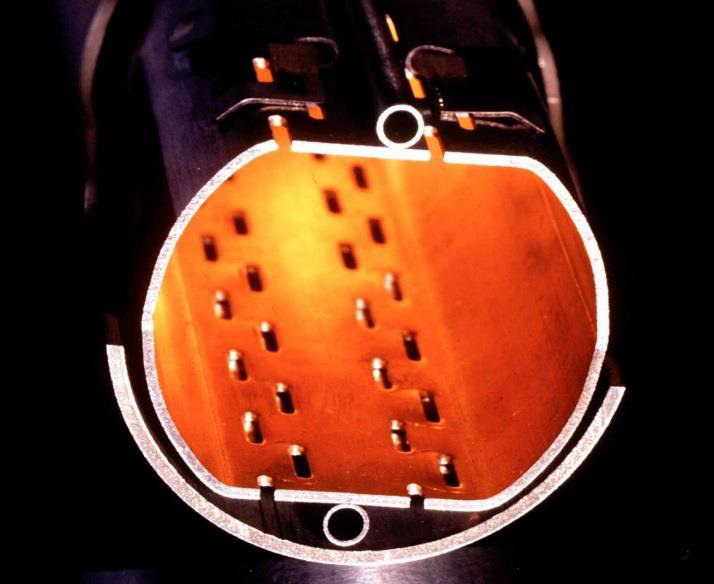
\includegraphics[width=\textwidth]{chapters/Chapter1/Figures/LHC_beam_screen.png}
    \end{subfigure}
    \begin{subfigure}{0.45\textwidth}
        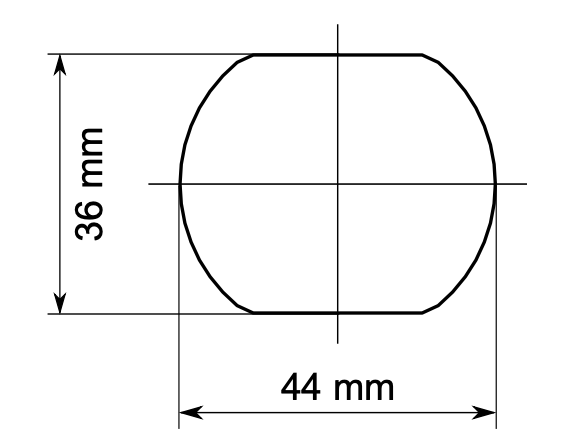
\includegraphics[width=\textwidth]{chapters/Chapter1/Figures/LHC_beam_screen_scheme.png}
    \end{subfigure}
    \caption{A section of the LHC beam screen.\cite{Iadarola:thesis}}
    \label{fig:LHCbeamscreen}
\end{figure}
In figure FIG we show the result of a very simple convergence study showing that the results obtained with the new solver are stable under mesh refinement.
\begin{figure}
    \centering
    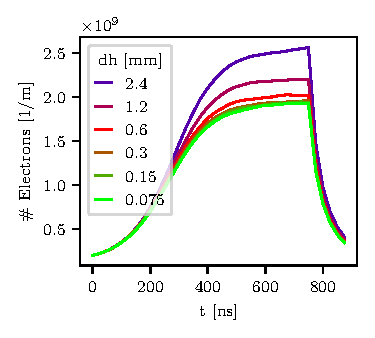
\includegraphics[scale = 1.4]{chapters/Chapter1/Figures/scan_dh.pdf}
    \caption{Results of the refinement study for the boosted frame electromagnetic solver in the LHC dipole case.}
    \label{fig:my_label}
\end{figure}
In Fig. \ref{fig:em_vs_es_dipole} we report a comparison of the evolution of the same buildup simulations with the electrostatic and the boosted-frame electromagnetic solver. 
\begin{figure}
    \centering
    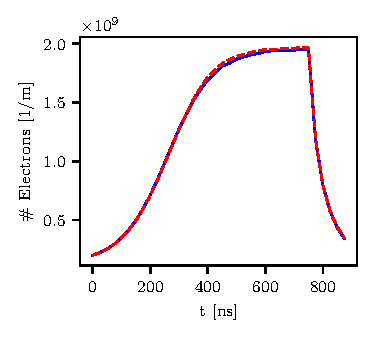
\includegraphics[scale=1.4]{chapters/Chapter1/Figures/em_es_comparison.pdf}
    \caption{Comparison of the buildup curves in an LHC dipole obtained with the electrostatic (red) and electromagnetic (blue) electrons space charge.}
    \label{fig:em_vs_es_dipole}
\end{figure}
The comparison shows that the results of the two types of simulations agree really well, which suggests that the effects of the magnetic field are negligible. In Fig. \ref{fig:es_vs_em_snap} we also show snapshots of the electrons distribution in the two cases.
\begin{figure}
    \centering
    \begin{subfigure}{0.47\textwidth}
        %\centering
        \hspace*{-2cm}
        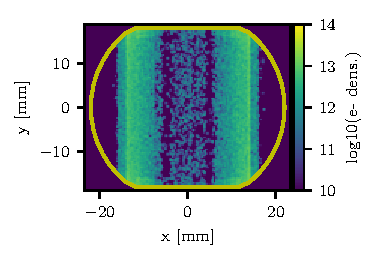
\includegraphics[scale=1.4]{chapters/Chapter1/Figures/es_dipole_snap.pdf}
    \end{subfigure}
    \hfill
    \begin{subfigure}{0.47\textwidth}
        %\centering
        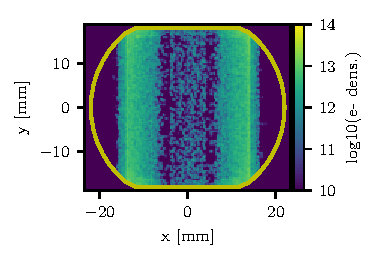
\includegraphics[scale=1.4]{chapters/Chapter1/Figures/em_dipole_snap.pdf}
    \end{subfigure}
    \caption{Snapshots of the electron cloud distribution in an LHC dipole using electrostatic (left) and electromagnetic (right) space charge fields.}
    \label{fig:es_vs_em_snap}
\end{figure}
To further understand the relevance of the magnetic fields in the electromagnetic simulations we analyze separately the contribution of the magnetic and electric fields to the force acting on the electrons. In order to do so we split Lorentz force
\begin{equation*}
    \mathbf{F} = q \left(\mathbf{E} + \mathbf{v}\times \mathbf{B}\right)
\end{equation*}
into the electric component
\begin{equation*}
    \mathbf{F}^E = q \mathbf{E},
\end{equation*}
and the magnetic one
\begin{equation*}
    \mathbf{F}^B = q \mathbf{v}\times \mathbf{B}.
\end{equation*}
The magnetic field plays a significant role in the dynamics of the electrons if the intensity of $\mathbf{F}^B$ is at least comparable to the one of $\mathbf{F}^E$, i.e. if $||\mathbf{E}||\approx||\mathbf{v}||||\mathbf{B}||$. To visualize the distribution of the two components of the Lorentz force, we compute them at the MPs positions as
\begin{equation*}
    \begin{split}
        \mathbf{F}^E_p &= q_p \mathbf{E}_p,\\
        \mathbf{F}^B_p &= q_p \mathbf{v} \times \mathbf{B}_p,
    \end{split}
\end{equation*}
and then we use the weighting area scheme to interpolate them at the mesh nodes. In Fig. \ref{fig:Fe_vs_Fb_snap} we report a snapshot of $\mathbf{F}^E$ and $\mathbf{F}^B$ during the gap between two bunches, which is when the space charge fields of the electrons are the most relevant. 
\begin{figure}
    \centering
    \begin{subfigure}{0.47\textwidth}
        %\centering
        \hspace*{-2cm}
        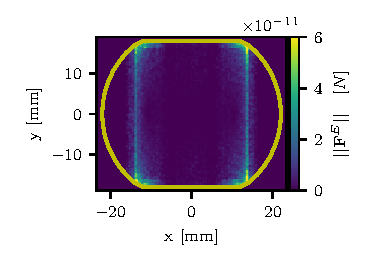
\includegraphics[scale=1.4]{chapters/Chapter1/Figures/Fe_Pass00028_00000.pdf}
    \end{subfigure}
    \hfill
    \begin{subfigure}{0.47\textwidth}
        %\centering
        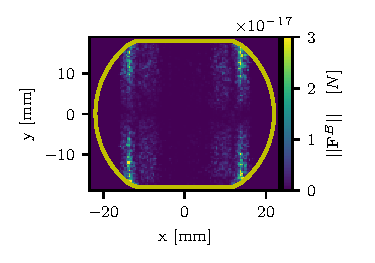
\includegraphics[scale=1.4]{chapters/Chapter1/Figures/Fb_Pass00028_00000.pdf}
    \end{subfigure}
    \caption{The distributions of $||\mathbf{F}^E||$ and $||\mathbf{F}^B||$ during the gap between two bunches.}
    \label{fig:Fe_vs_Fb_snap}
\end{figure}
The space distribution of the two forces is essentially the same, but the electric component is six orders of magnitude more intense then the magnetic one, showing that the magnetic effects can be neglected. In Fig. \ref{fig:Fe_vs_Fb_hist} we also report (smoothed) histograms of the forces on the MPs during the passage of a bunch and during the gap between two bunches.
\begin{figure}
    \centering
    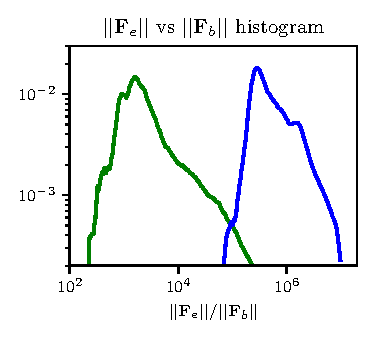
\includegraphics[scale=1.4]{chapters/Chapter1/Figures/Fe_Fb_hist.pdf}
    \caption{Caption}
    \label{fig:Fe_vs_Fb_hist}
\end{figure}
During the passage of a bunch the magnetic force is closer in magnitude to the magnetic one, which is expected because the electrons move faster, but it is still three orders of magnitude lower than the electric one. All in all, we can conclude that the magnetic component of the space charge Lorentz force is so low that it can be neglected, confirming that the space-charge fields of the electrons can be computed in the electrostatic approximation.

